\documentclass[aps,letterpaper,11pt]{revtex4}
\usepackage{graphicx} % For images
\usepackage{float}    % For tables and other floats
\usepackage{verbatim} % For comments and other
\usepackage{amssymb}  % For more math
\usepackage{fullpage} % Set margins and place page numbers at bottom center
\usepackage{listings} % For source code
\usepackage[usenames,dvipsnames]{color} % For colors and names
\usepackage[pdftex]{hyperref}           % For hyperlinks and indexing the PDF
\usepackage{pdfpages}
\usepackage{subfig}
\usepackage{listings}
\usepackage[usenames,dvipsnames,svgnames,table]{xcolor}
\usepackage{color}
\usepackage{textcomp}
\usepackage[utf8]{inputenc}
\lstset { %
    language=C++,
    backgroundcolor=\color{black!5}, % set backgroundcolor
    basicstyle=\footnotesize,% basic font setting
}
% Custom colors
\definecolor{deepblue}{rgb}{0,0,0.5}
\definecolor{deepred}{rgb}{0.6,0,0}
\definecolor{deepgreen}{rgb}{0,0.5,0}

 \lstset{
  tabsize=4,
  language=C++,
  captionpos=b,
  tabsize=3,
  numberstyle=\tiny,
  numbersep=5pt,
  breaklines=true,
  showstringspaces=false,
  basicstyle=\footnotesize,
%  identifierstyle=\color{magenta},
  keywordstyle=\color[rgb]{0,0,1},
  commentstyle=\color{deepgreen},
  stringstyle=\color{deepred}
  }
  
\hypersetup{ % play with the different link colors here
    colorlinks,
    citecolor=black,
    filecolor=black,
    linkcolor=black,
    urlcolor=blue % set to black to prevent printing blue links
}

\newcommand{\labno}{Software Engineering Project}
\newcommand{\labtitle}{Final Report}
\newcommand{\authorname}{Group members:\\Antoine Merlet\\Gülnur Ungan\\Mladen Rakic\\Marcio Aloisio Bezerra Cavalcanti Rockenbach}
\newcommand{\professor}{Dr. Yohan Fougerolle, Dr. Cansen Jiang, Dr. David Strubel}


\begin{document}
\begin{titlepage}
\begin{center}
{\LARGE \textsc{\labno:} \\ \vspace{4pt}}
{\Large \textsc{\labtitle} \\ \vspace{4pt}} 
\rule[13pt]{\textwidth}{1pt} \\ \vspace{150pt}
\begin{figure}[!htb]
  
\includegraphics[scale=1.0]{logo.jpg}
\end{figure}
{\large \authorname \\ \vspace{10pt}
Professors: \professor \\ \vspace{10pt}
\today}
\end{center}


\end{titlepage}% END TITLE PAGE %%%%%%%%%%%%%%%%%%%%%%%%%%%%%%%%%%
\newpage

\tableofcontents

\pagebreak
\setlength{\parindent}{10ex}
\setlength{\parskip}{1em}

\section{Introduction / Context}
This project is the main assignment of the Software Engineering course, which belongs to the first semester of the University of Burgundy Masters programs MAIA, ViBOT and MsCV. The course is taught and mentored mainly by professor Yohan Fougerolle, accompanied by Mr David Strubel and Mr Cansen Jiang. Our group is made out of four members, namely Gulnur Ungan, Antoine Merlet, Marcio Rockenbach and Mladen Rakic. All of our group members are from the MAIA Program, each of us with different backgrounds. That versatility and the individuality of all the team members were the key ingredients in making this project a reality.\par
The proposal of the project was to work on improvements of the previous year projects regarding the development of a software that scans a person using an external sensor (Kinect v2) and captures and displays a 3D representation of the scanned model. Although the previous year’s students achieved relatively acceptable results, there are still many implementation flaws and much room for improvement. The codes and the reports were difficult to read and understand, the implementation was lacking some common programming practice and the installation process was quite challenging. Throughout this report, we will discuss the goals and main targets for improvement decided by the group, ways of achieving them and main challenges faced, the results we accomplished and propositions on what can be done in the future development.\par
\pagebreak

\section{Choices / Target}
In terms of defining the main goal we want to achieve, we analyzed the target through various aspects. We believe that these points are very important when it comes to general improvement of the project and to better understanding of it for the next generation of students. Namely, these aspects can be formulated as follows:
\begin{itemize}
  \item We decided to make the user interface in a way that is more readable and understandable (i.e. more user-friendly). The way to accomplish this is to create GUI based on forms instead of creating the blank GUI and then implementing separate elements manually. We argue that this way makes it easier to manage, modify and improve individual components of the GUI in comparison to the manual implementation.
  \item Organization of the code is another major point we wanted developed, meaning that the code, which is split into several modules, is more suitable for corrections and overall understanding. Our implementation should also be, for the most part, non-Qt dependant and also non-PCL dependant, which is a significant improvement, since it allows someone to easily switch to implementation using OpenCV, for example.
  \item Interfacing is another thing we want to advance, in a sense that the user interface is supposed to be very simple and minimalistic in design, yet very powerful, offering a wide range of options and methods for the user to choose from. Those methods, being very advanced, still should not add to the complexity of the interface usage. User manual is a particularity which ought to make things easily comprehensible.
  \item One of the most important milestones we wanted to reach is a good documentation of the project. This can be obtained through several instances - well commented code; logger class which helps a lot with most of the debugging processes and also adds to the overall user-friendliness; functions that are separately and precisely documented; overall good coding habits, such as reasonable naming of the functions, classes and variables and consistency throughout all the files; the manuals and the diagrams to make the project easily and relatively quickly readable and understandable; etc. 
  \item We want to offer a wide palette of various filtering and registering options to choose from, rather than to stick to ICP only. We also aim to allow a reasonably effortless and straightforward refinement of the parameters, a crucial thing for the following generation that will possibly build upon our project.
  \item Considering the amount of the workload and the functionalities we focused on, it remains to be said that our main target was not to improve the meshing part of the project. Regarding that, we argue that having provided the good interfacing, methods for filtering and registration, debugging tools and overall organization and documentation of the code, it is significantly less demanding to build upon the current state of the project and provide a good meshing algorithm than it would be in any other scenario.
\end{itemize}\par
All the bullet points stated above serve to justify one of the most important decisions we made, which is to actually start the whole project from scratch. We firmly believe that, taking the current state of the previous year’s projects, it is a wise choice to accept and keep some of the things we think are fairly well developed, and incorporate them intact or modified into our project, but all the time sticking to our goals and the way of organizing it. \par
\pagebreak

\section{Project Management}
To implement the difficult goal of carrying out this project, we decided to split it in different tasks. The idea was to assign the tasks in such a way that they are as much independent from each other as possible, making the overall management and individual development smooth. The rough assignment of the objectives is the following:
\begin{itemize}
\item Antoine: overall project design
\item Marcio: input and output of the data
\item Gülnur: filtering and registration techniques
\item Mladen: GUI
\end{itemize}\par
Even though the assignments appear very individual and distinct from each other, we had to have good organization and communication skills in order to link all the dots properly and put the whole project into practice.\par
We created a repository for our group in that can be found in GitHub (\url{https://github.com/AntoineMerlet/3DScan}), in which we kept all the source codes and other important files. We had weekly group meetings to discuss everyone’s progress and to address difficulties encountered, as well as to further develop the future assignments. Those meetings were always documented in our repository. Also, everyone had a personal weekly report, where each of us made a description on what we had worked on and the future tasks. More detailed description of each individual task will be provided in the upcoming sections.\par

\subsection{Antoine}
\subsection{Marcio}

\subsubsection{Logger}
One of my main goals was to create a logger class, responsible for creating and managing a log, which registers all the main important events that occur when a software is running. Through that tool, it is much easier to debug the code. That being said, it represents a significant improvement in comparison with previous year's projects. We can insert log messages in the chosen key points in the source code and then analyse its behaviour through the log.\par
In our software, I implemented the log in a singleton design, which means that it restricts the instantiation of a class to a single object, created in the main window. This pattern is useful in our case because we want the same logger to be called by all the windows and classes in our program.\par
The logger then operates through a pointer, which represents the only instance of the class, as stated before. First, for every session of the program, a .txt file is created in the build directory. The name of the file is as follows: Log + CurrentDate + CurrentTime + .txt. After the initiation of the logger, we also connect the pointer to the main window through a QTextEdit using Qt signals / slots system. This widget is constantly updated to display all the messages sent to the logger (figure \ref{fig:logger}).\par
\begin{figure}[h]
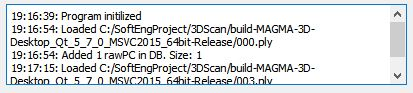
\includegraphics[scale=1]{logger_mw}
\caption{Logger widget in the main window}
\label{fig:logger}
\end{figure}

I also implemented the logger in a way that is easy to be used everywhere in the code. This was done by defining a macro. By simply typing LOG(-- string message here --); in any part of the code, we can send a message to be included in the log file. Although this is not the most secure way to implement it(since it is not type safe), it adds a lot to easiness of usage. This class definitely can and should be improved by next year students, but it already is a functioning tool for project debugging.\par

\subsubsection{I/O Tools}
My second goal was to handle most of the input and output section of our project. For that, I had to work with the Kinect sensor and to implement the necessary code to obtain and save data from the Kinect and to display the point clouds in a visualizer.\par
The Kinect for Windows version 2.0 was released in the end of 2013 / beginning of 2014. The sensor is composed of an RGB camera (3 channels) that stores data in a 1280 x 960 resolution, an infrared emitter and an infrared depth sensor, which allows it to capture a depth image with resolution of 512 x 424. It also features a microphone and an accelerometer. It has a depth range between 0.4 - 4.5 m and has a field of view 70º horizontally and 60º vertically.\par
Point cloud library (PCL) has some modules for data input that are called grabbers, but it does not have one specific for the Kinect. Although it is not implemented in the PCL itself, previous year projects made use of a grabber for the Kinect that is available on the internet (\url{http://unanancyowen.com/en/pcl-kinectv2-with-grabber/}) and that is implemented in only one header / cpp file. We decided to keep this method of data acquisition by using this class.\par
After implementing and testing the Kinect acquisition using the kinect2grabber, it was necessary to connect it to our project. I worked with Mladen in the development of the GUI for that purpose, by creating a PCL Visualizer to display the live scan. For the acquisition of the point clouds, I implemented a callback function that interacts with the keyboard. By pressing the key “s”, one point cloud is stored in the system. The visualizer of the live scan also features a bounding box, whose coordinates can be determined through sliders in the scan window.\par
I also worked on the loading and display of the point clouds in the main window (figure \ref {fig:PCdisp}). When the user selects the files to be loaded, a QListView widget is updated to display the corresponding filenames. By interacting with this widget (by checking or unchecking the items), the display widget (a QVTK widget) is updated to show the selected point clouds.\par

\begin{figure}[h]
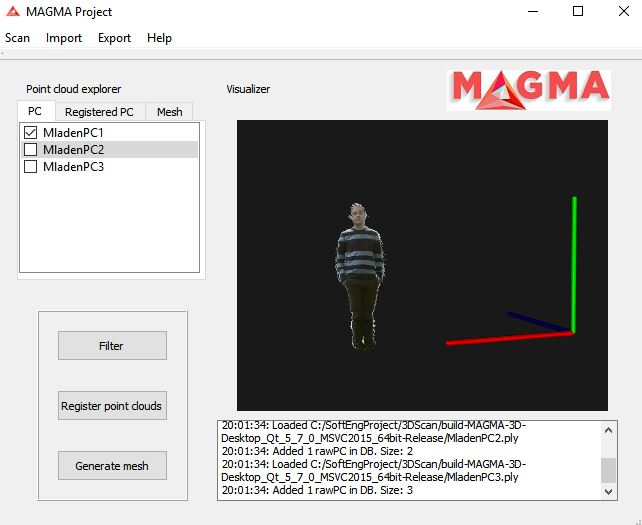
\includegraphics[scale=0.5]{PC_display}
\caption{Display of point clouds}
\label{fig:PCdisp}
\end{figure}

Since the input and output are closely related to interaction with the user, it was a good opportunity for me to also learn a lot about GUI design in Qt and how to transmit information between different modules of the software.\par

\subsection{Gülnur}
\subsection{Mladen}
One of the main reasons that made me tackle this particular part of the project was to actually get familiar with the concepts of creating the user interface and to get a better understanding of the way components are organized and connected. Also, the ability to design things in an appealing, yet simplistic and minimalistic way, came in handy when it came to this. Having studied the previous year’s designs of the interface, I found numerous flaws in both the aesthetics and the implementation. Therefore, the proposed GUI, even though it inherited some minor concepts from those, is for the most part built from scratch and developed in a way to suit the particular needs of our proposal.\par
The principal concept around which the whole design process revolved is to make the interface as much user-friendly as possible, while keeping it powerful, in a sense that it is able to provide the user with the wide variety of methods and parameters choices. The way I implemented this was to create several independent windows, each serving a particular purpose, while maintaining the user not overwhelmed with the amount of content.\par
Another salient aspect was to implement the overall connectivity between the GUI and other classes in a way that makes them as much independent from each other as possible. This is a powerful way to make the code easily modifiable and it will be further elaborated in this section. Although one might argue that some of it might not be the most elegant or the most common programming practice, we have to bear in mind that this way puts the project in a state that is very understandable and readable, which is very convenient for the next generation of students.\par
The user interface is consisted of a number of key components. These can be listed as follows:
\begin{itemize}
\item Main window, which gives user the possibility to interact with the major functionalities, such and importing and exporting of the point clouds, filtering and registering the data, generating the mesh, as well as the access to the user manual and the about section. Another particularity which makes the experience more user-friendly is the logger, implemented by Marcio, which helps to keep the track of the ongoing and completed processes, and serves as a great tool for the debugging. 
\item Scan window, used to perform live scans directly from the Kinect sensor. Other than that, it enables easy manipulation of the bounding box on the live scan which should bound the sensor’s field of view. It also allows the easy capturing of the raw point clouds and has a variety of options for further development, such as the choice of performing horizontal or vertical acquisition. This, however, will be further developed in the Future tasks section. 
\item Filter window, which is a dialog box for an easy selection of the filters and the corresponding parameters. 
\item Register window, which is yet another dialog box that offers a variety of the registration methods and choosing of their respective parameters. 
\item About section, a pop-up window with the basic information regarding the project, team members, and mentors.
\end{itemize}\par
To further elaborate the overall design and implementation, and to justify some of the choices I made, I will make a brief insight on some key concepts. Main window (figure \ref {fig:wind1}), however simple it may seem, offers an access to all the parts of the project very easily. It allows the user to load or save the point clouds and to display them on the QVTK Widget. It is possible to choose from a list of the loaded point clouds and to display multiple point clouds at once. The list of the point clouds with the checkboxes makes the whole process very intuitive and reasonable. \par
Clicking on a new scan option opens up the scan window (figure \ref {fig:wind2}), while at the same time hiding the main window, which is a redundant component when it comes to the new acquisition. Scan window manages the manipulation of the bounding box and the capturing of raw point clouds from live feed from the sensor. Stopping the scan and closing the scan window make the main window appear again, with all the finished processes stated in the logger.\par

\begin{figure}[!htb]\centering
   \begin{minipage}{0.49\textwidth}
     \frame{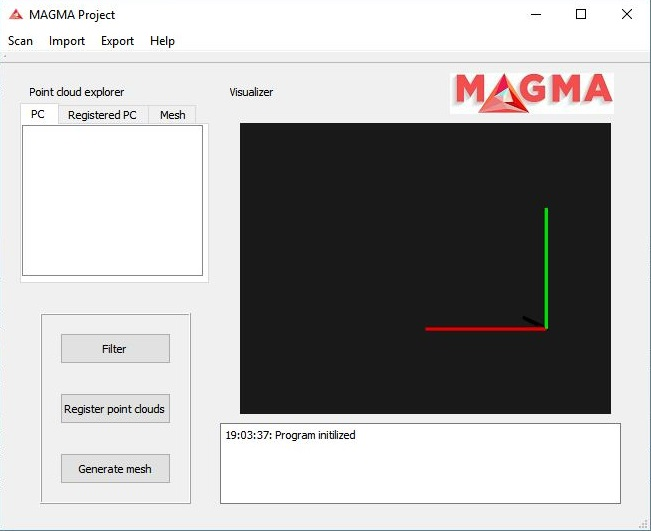
\includegraphics[width=\linewidth]{main_window}}
     \caption{Main Window}\label{fig:wind1}
   \end{minipage}
   \begin {minipage}{0.49\textwidth}
     \frame{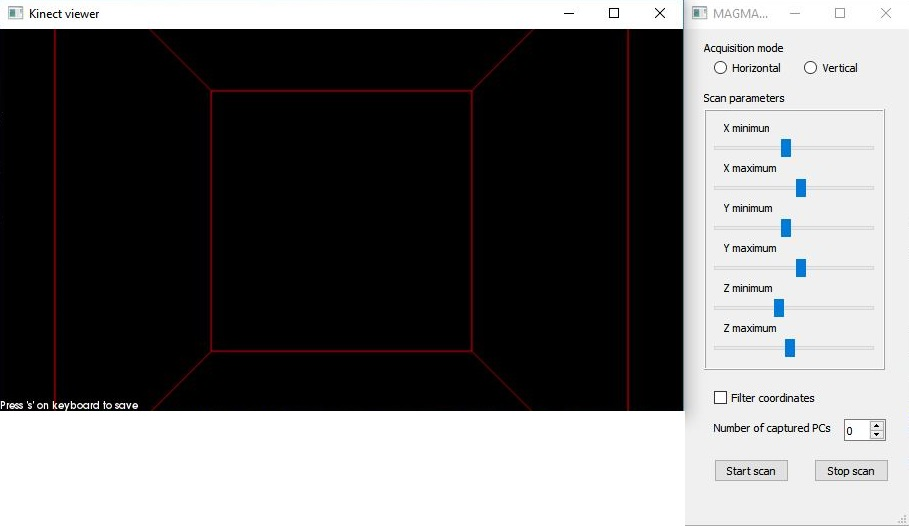
\includegraphics[width=\linewidth]{scan_window}}
     \caption{Scan Window}\label{fig:wind2}
   \end{minipage}
\end{figure}

As previously stated, some of the choices I made may not seem reasonable or elegant, and that is regarding the filtering and the registration windows (figures \ref{fig:wind3} and \ref {fig:wind4}, respectively). Namely, both of those windows contain numerous methods for data processing and the corresponding parameters which can be chosen. All the storage of the data is handled by the structures that contain them. For instance, parameters for median filter  are stored into the following structure:\par
\begin{lstlisting}
       struct median {
       bool checked = false;
       int windowsize;
       int maxmovement;
   	   } medianfilt;
\end{lstlisting}\par
Member \textit{checked} serves to store the information whether the corresponding checkbox on the filter window has been checked or not. Clicking on the Filter button will trigger a function that will check which boxes have been selected by the user, then switch the \textit{checked} member of the corresponding structure to true and then and only then allow the storing of the parameters for that particular structure. That way, when the filtering parameters are chosen and the window has been closed, the appropriate function that performs the filtering will be able to accept the parameters only from the structures that have the member \textit{checked} set to be true. This implementation makes the user interface fairly independent from the mathematical tools (filtering and registration functions) and makes it easy to potentially modify the parameters and the used methods themselves. I can argue that this way is well suited for the refinement and further improvement of the data processing. It certainly made the project management simple in a sense that big parts we all individually worked on, although very connected and dependent when considering the project as a whole, can still be partially independently developed.\par

\begin{figure}[!htb]\centering
   \begin{minipage}{0.49\textwidth}
     \frame{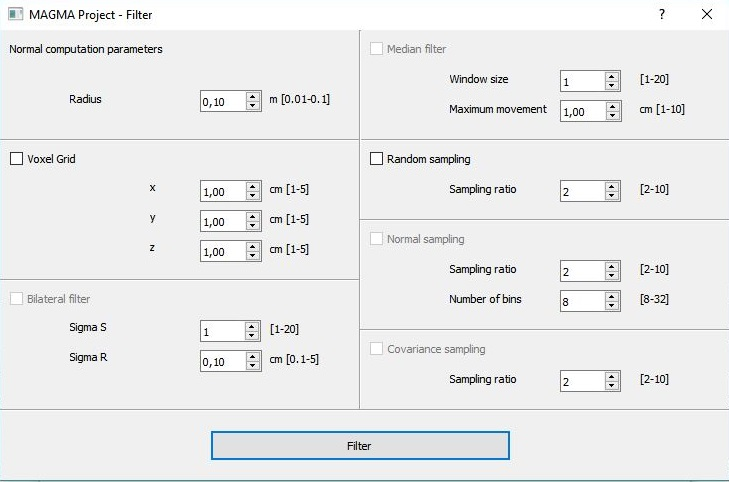
\includegraphics[width=\linewidth]{filter_window}}
     \caption{Filter Window}\label{fig:wind3}
   \end{minipage}
   \begin {minipage}{0.49\textwidth}
     \frame{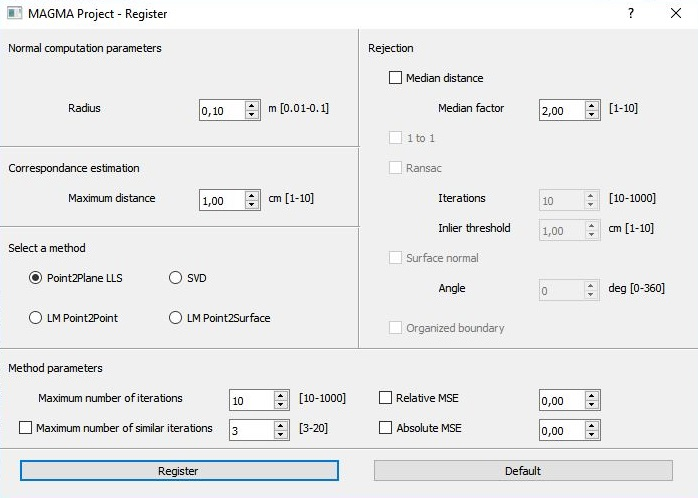
\includegraphics[width=\linewidth]{register_window}}
     \caption{Register Window}\label{fig:wind4}
   \end{minipage}
\end{figure}


\pagebreak

\section{Challenges}
One of the main challenges to start to work on this project is the simple installation and configuration of the source code. Since it requires different libraries which need to be correctly installed and configured both in the user's system and in the project files, it is a very time consuming task. It takes a lot of effort to download all of the required tools and to make them work. Because of that, we needed weeks just to be able to run the previous year projects and to start working on improvements.\par
Other important challenge is to learn the “Qt ways”. Qt is a very powerful tool, but requires a lot of time and studying to learn and to be comfortable with its syntax and methods. For example, Qt has an option to implement GUI using forms and it also uses a signals / slots system to make it easier to communicate between different objects in the software. Those are great features, but the majority of our group was not familiar with that before the project started.\par
Finally, one of the most significant challenges is the level of complexity of the project. It is a huge leap between small console oriented projects using only basic C++ syntax and STL that we did in the labs and in class to a elaborate project involving user interface, usage of different and complex libraries and interaction with an external sensor.\par
\pagebreak

\section{Conclusion}
Taking into consideration all the bullet points stated in Target section, as well as the elaborations of the individual and the group work on the project, we can conclude that we managed to reach the goal that was set. We can justify this statement by making a brief resume of the accomplished objectives. We did manage to build a GUI based on forms instead of a manual implementation, which makes it way more understandable and easier to manipulate. Also, we strongly argue that our code organization is well executed, in a sense that it is well organized and structured, documented and commented, with all the necessary diagrams, manuals and debugging tools to make the user experience pleasant. The code, and the project as a whole is quite consistent and undemanding to follow - this makes the reverse engineering for the next generation a reasonably fair task.\par
We did not, however, implement the meshing part, but the current state of the project is a fairly good platform to build upon. Parameter refinement is easily achievable, different modules of the project are as independent as possible, which makes the software understandable and improvable. Another good argument to support the idea of the project being a good platform to build upon is the fact that the mathematical tools implemented offer a wide variety of methods for filtering and registering and one might decide on the optimal ones fairly easy, and develop on that. \par
To conclude, even though the project was started from the scratch, and even though our skillset and the given amount of time are arguably insufficient, the current stage the project is at is very noteworthy and remarkable. 
\pagebreak

\section{Future Work}
For the next generation of students who will work on this project, we propose some improvements that can be done on the software:\par
\begin{itemize}
\item Logger: implementation without using macro, making it typesafe
\item Implement meshing techniques of the registered point clouds
\item Horizontal / vertical acquisition modes: allows the user to choose between vertical and horizontal orientation of the Kinect sensor.
\item Save captured files in other extension than “.PLY”
\item Full implementation of the software as Qt and PCL independent
\end{itemize}


\pagebreak

\section{References}
\begin{enumerate}
\item \url{http://unanancyowen.com/en/pcl-kinectv2-with-grabber/}
\item \url{https://github.com/UnaNancyOwen/KinectGrabber/tree/Kinect2Grabber/Sample}
\item \url{https://cppcodetips.wordpress.com/2014/01/02/a-simple-logger-class-in-c/}
\item \url{http://pointclouds.org/}
\item \url{https://www.vtk.org/}
\item \url{http://zugara.com/how-does-the-kinect-2-compare-to-the-kinect-1}
\item \url{https://github.com/umaatgithub/3D-KORN}
\item \url{https://github.com/WajahatAkhtar/Project-S.E}
\end{enumerate}





\end{document} % DONE WITH DOCUMENT!

